
\chapter{Généralités}
\section{Introduction}
Une conception parfaite dès le premier coup n’existe pas, ce qui fait de la tâche de conception une tâche itérative. Les concepteurs avec l’expérience ont remarqué qu’il y a quelques choses qui se répètent d’une conception à l’autre, ce qui a donné naissance à la notion de « patron » et « anti patron » de conception.
\vspace{5px}\\
Dans ce chapitre, nous présentons les patrons et les anti-patrons de conception et nous citons les approches utilisées pour détecter ces anti-patrons.

\section{Les patrons de conception}
La notion de patron de conception est apparue avec les travaux de \cite{alexander1977pattern} dans le domaine d’architecture, et depuis, ce même concept a été appliqué dans le domaine de gestion de projet et de la conception de logiciels informatique à laquelle nous nous intéressons dans ce rapport. \newline
Les patrons de conception orientée objet ont été popularisés avec la publication en 1994 du livre : Design Patterns : Elements of Reusable Object Oriented Software \cite{vlissides1995design} qui est un catalogue de patrons de conception indépendant du langage de programmation. \newline
Un patron de conception est défini comme étant une solution générale à un problème récurrent dans un contexte particulier. Un patron de conception est décrit avec quatre éléments \cite{vlissides1995design}:
\newline
\begin{itemize}
   

  \item Le nom du patron : qui peut repérer le problème et la solution, est le moyen de communication entre les développeurs concernant ce patron.
  \item Le problème : décrit le contexte ou la situation dans laquelle le patron s’applique.
  \item La solution : décrit les éléments de la conception qui règlent le problème détecté, indépendamment de l’implémentation et du langage, qui peut être utilisée dans d’autres situations.
  \item Les conséquences : décrit les résultats de l’application du patron et son impact sur la flexibilité et l’extensibilité de la solution.
\end{itemize}
\newline
Les patrons de conception sont catégorisés sous trois types selon leur mission :
\begin{itemize}
    \item Patrons de création: Exemples; Abstract Factory, Builder, Factory.
    \item Patrons de comportement: Exemples; Adapter, Bridge, Composite.
    \item Patrons de structure: Exemples; Interpreter, Iterator, Mediator.
\end{itemize}
\section{Les anti-patrons de conception et les code smells}
Ce terme introduit pour la première fois par Koenig en 1998, veut dire les mauvaises solutions récurrentes à des problèmes de systèmes logiciels \cite{brown1998antipatterns}. Il est important pour les développeurs de connaître les anti-patrons, pour savoir les situations où une solution peut avoir un impact négatif et donc l’éviter, parmi les anti-patrons les plus connus, nous citons: Blob, Spaghetti Code, Swiss Army Knife.
\newline
Afin de détecter les anti patrons, des symptômes ont été recensés, appelées, code bad smells, qui représentent des signes de manifestation dans le code source qui aident à mieux trouver les parties de code pouvant contenir des anti-patrons.
\newline
Ils sont catégorisés selon \cite{mantyla2003taxonomy} sous six groupes (sauf deux smells qui ne rentrent dans aucun groupe qui sont: Incomplete Library Class et Comments) afin de comprendre la relation entres les code smells de même groupe et trouver les corrélations entre eux pour optimiser l'étape de refactoring:
\begin{itemize}
    \item \textbf{The Bloaters} : englobent les code smells qui caractérisent les classes et méthodes qui sont très grandes et difficilement maintenables, par exemple: Long Method, large class qui implique l’existence de l’anti-patron Blob, Primitive Obsession ou Long Parameter List.
    \item \textbf{The Object-Oriented Abusers} : englobent les code smells qui caractérisent des cas où les principes orientées objet ne sont pas respectés (polymorphisme, encapsulation...etc.) par exemple: Switch Statement qui peut être transformé en exploitant le polymorphisme, le bad smell Poor Usage of Abstract Classes.
    \item \textbf{The Dispensables} : englobent les code smells qui caractérisent les classes supplémentaires, qui ne jouent presque aucun rôle dans le code, par exemple :Lazy Class,Data Class
    \item \textbf{The Couplers} : ce sont les défauts de conception qui augmentent le couplage entre les classes, exemples :Law of Demeter
    \item \textbf{The Encapsulators} : englobent les code smells qui ont une relation avec les mecanismes de communication et d'encapsulation des données dans le code source, par exemple, le code smell Message Chains .
    \item \textbf{The Change Preventers} : englobent les code smells qui impliquent, en cas de modification dans le code source, que soit une classe doit être modifiée suite à plusieurs types de modification comme le code smell Divergent Change ou bien plusieurs classes à modifier au cas d'un seul changement comme le code smell Shotgun Surgery, parce que , les modifications possibles doivent avoir une relation 1-1, c'est à dire, un seul changement implique la modification d'une seule classe.
\end{itemize}
\vspace{1cm}
La compréhension des causes d'apparition des anti-patrons est aussi importante que son étude, c'est pourquoi, nous citons ici les causes principales qui peuvent engendrer un anti-patron de conception\cite{brown1998antipatterns}:

\begin{itemize}
\item  La conception sous des contraintes de temps : le but dans ce cas est de réaliser quelque chose de fonctionnel, mais pas nécessairement maintenable ou de qualité.
\item Le changement continu du code : sans comprendre le code surtout par des développeurs différents de ceux qui ont écrit le premier code source.
\item Le non-respect des bonnes pratiques de conception et de codage.
\item L’ignorance et/ou la fierté des développeurs : ne pas commenter son code ou ne pas bien écrire ses commentaires est l'un des exemples les plus simples de ce cas.
\end{itemize}
\vspace{1cm}
Un autre aspect à aborder concernant les anti-patrons, c'est la documentation, qui est très importante pour permettre la communication facile entre les développeurs, et comme les patrons, les anti-patrons ont leur propre documentation aussi qui figure sous plusieurs formes :
\begin{itemize}
    

    \item \textbf{La pseudo-documentation}: donne le nom et le problème de l’anti-patron en question.
    \item \textbf{La mini-documentation }: fournit le nom de l’anti-patron, le problème et la solution proposée.
    \item \textbf{La documentation complète}: contient le nom le plus connu, les autres noms s’il en existe, contient aussi le niveau fréquent auquel  cet anti-patron peut être détecté(niveau application,micro architecture ou framework..etc) , le nom de la solution et son type, les forces déséquilibrées qui ont été sous-estimées comme la gestion de fonctionnalités ou gestion de complexité, la forme générale de l’anti-patron donnée sous forme de diagramme, symptômes et conséquences, aussi les exceptions connues où cet anti-patron n’a pas d’impact négatif, d’autres anti-patrons liés à l’anti-patron en question, exemple et applicabilité à d’autres niveaux.
\end{itemize}
\vspace{1cm}
Dans la figure \ref{fig:patanti} ci-dessous, \cite{brown1998antipatterns} illustre la relation entre les patrons et les anti-patrons.

\begin{figure}[H]

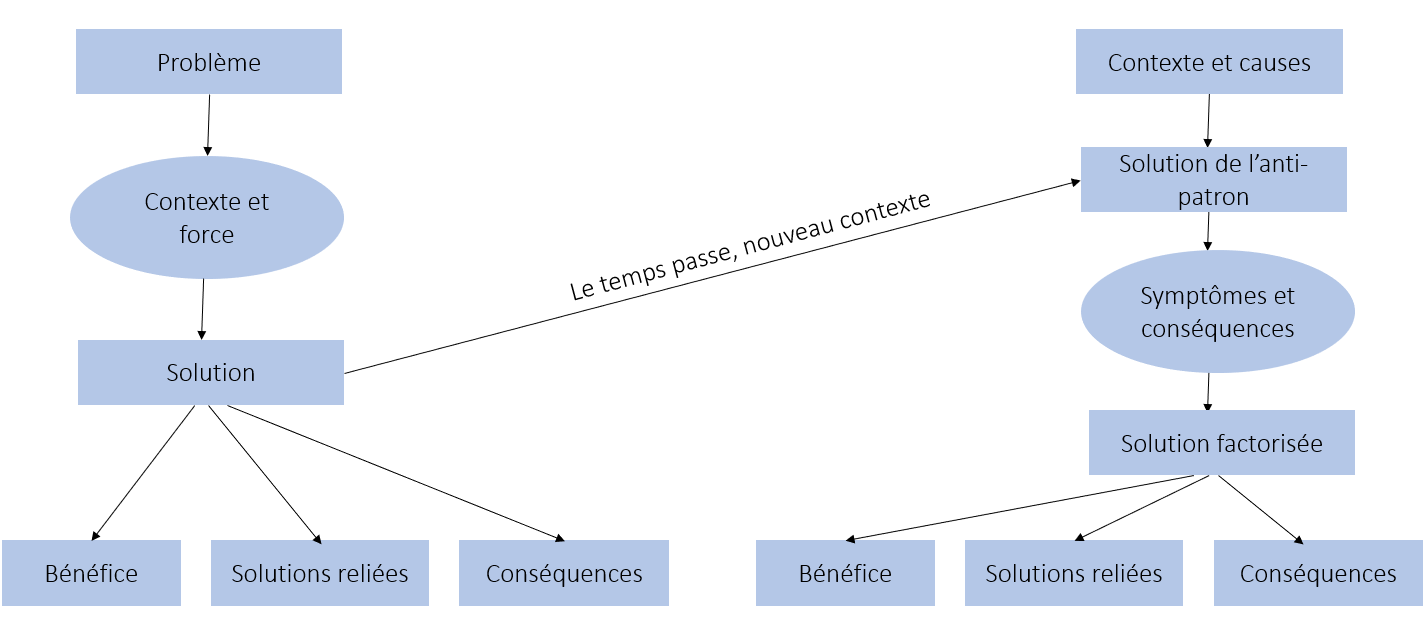
\includegraphics[width=\textwidth]{Others/Resources/patronetantipatron.PNG}
	\caption{La relation entre les patrons et les anti-patrons \cite{brown1998antipatterns}.}
		\label{fig:patanti}
	\end{figure}
	
	\section{Détection  des anti-patrons de conception}
	Dans ce paragraphe, nous présentons brièvement les différentes approches de détection des anti-patrons qui existent déjà dans la littérature.
	
	\cite{travassos1999detecting} ont introduit un processus basé sur les inspections manuelles et les techniques de lectures afin d’identifier les mauvaises odeurs du code. Aucune tentative n'a été réalisée pour automatiser ce processus, et par conséquence, la technique resterait difficilement applicable sur les systèmes logiciels compliqués.
\cite{marinescu2004detection} a présenté une approche basée sur les métriques pour détecter les odeurs de code avec des stratégies de détection. Cette approche est mise en œuvre via l'outil IPLASMA. La stratégie consiste à capter à l'aide des métriques, les écarts par rapport aux bons principes de conception, ensuite elle combine ces métriques avec des opérateurs  et compare leurs valeurs par rapport à des seuils absolus et relatifs.
\cite{munro2005product} a remarqué les limitations des descriptions textuelles et a proposé un modèle pour décrire les odeurs de code systématiquement. Ce modèle est similaire à celui utilisé pour les patrons de conception \cite{vlissides1995design}. Il se compose de trois parties principales : le nom de l'odeur de code, la description textuelle de ses caractéristiques et les heuristiques utilisées pour sa détection.
\newline
Ce travail est considéré comme un pas vers des spécifications plus précises des odeurs de code. Munro a également proposé des heuristiques basées sur les métriques pour détecter les odeurs de code, qui sont similaires aux stratégies de détection de Marinescu. Il a également effectué une étude empirique pour justifier le choix des métriques et des seuils de détection des odeurs.
\newline
\cite{alikacem2009metric} ont proposé un langage pour détecter les violations des principes de qualité et des odeurs dans les systèmes orientés objets. Ce langage permet la spécification de règles en utilisant les statistiques, l'héritage ou les relations d'association entre classes, selon les attentes des ingénieurs. Il permet également d'utiliser la logique floue (fuzzy logic) pour exprimer les seuils de règles conditions qui sont exécutées par un moteur d'inférence. Quelques approches traitant les systèmes complexes utilisent les techniques de visualisation \cite{dhambri2008visual}, \cite{simon2001metrics}, telle que les approches semi-automatiques qui sont intéressantes comparées avec les techniques automatiques qui peuvent être efficaces  mais perdent la trace du contexte et l'inspection manuelle est lente et inexacte \cite{langelier2005visualization}, de plus, elle
nécessite une expertise humaine et donc encore plus de temps. 
\newline
D'autres approches de détection fonctionnent entièrement d’une façon automatique pour détecter des odeurs de code et utilisent les techniques de visualisation pour présenter les résultats de la détection \cite{lanza2007object}, \cite{van2002java}.
D'autres approches connexes incluent les détecteurs de cohérence architecturale, qui ont été intégrées dans les environnements architecturales de développement \cite{garlan1995architectural}, \cite{allen1997formal},\cite{dashofy2005comprehensive}.
Par exemple, les agents actifs agissant comme des critiques \cite{dashofy2005comprehensive} qui peuvent vérifier les propriétés des descriptions architecturales, identifier les erreurs syntaxiques et sémantiques potentielles et les signaler au concepteur.
Toutes ces approches ont contribué d’une manière significative à la détection automatique des odeurs. 
